%!TEX root = ../../main.tex
\section{Discussion}
\label{sec:Discussion - Dose Decay Modelling}
The DWD is a dose metric that was introduced by Zeldin \textit{et al.} which represents ``the average dose in the diffracting crystal volume from which the photons making up a given image have scattered'' \cite{zeldin2013dwd}.
In essence, the DWD is a weighted average of the dose where the weights are given by the fluence at each point in the crystal (equation \ref{eq:DWD equation - no RDE}).
Zeldin \textit{et al.} demonstrated that DWD was superior to other metrics (average dose - whole crystal and the maximum dose) in predicting the relative intensity loss of protein crystals whilst accounting for different beam profiles.
\begin{figure}
  \centering
    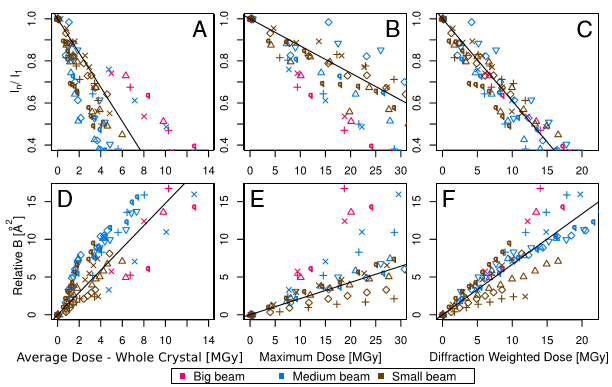
\includegraphics[width=1\textwidth]{figures/dwd/zeldin_metric_comparisons.png}
    \caption[Dose metric comparison: DWD, Average dose (whole crystal) and Maximum dose]{(A-C) $I_n/I_1$ against dose.
    The reduced scatter along the line of best fit in (C) is evidence that DWD is invariant to the dose distribution in the crystal.
    (D-F) $B_{rel}$ against dose.
    There is no obvious reduction in scatter around the line of best fit for these metrics.
    This suggests that DWD offers no significant improvement over other dose metrics when using $B_{rel}$ as a measure of radiation damage progression.
    The symbols represent individual crystals.
    Reproduced from \cite{zeldin2013dwd}.}
    \label{fig:Dose metric comparisons - zeldin et al}
\end{figure}
The improvement in relative intensity decay prediction makes DWD a promising metric for comparing radiation damage studies and also for zero dose extrapolation.
However, data points are still scattered around the line of best fit in Figure~\ref{fig:Dose metric comparisons - zeldin et al} (C).
The scatter is thought to be caused by two factors:
the first is the intrinsic variation in crystal quality, and the second is the fact that the DWD does not account for the effects of inhomogeneous dose distribution, such as an uneven loss of diffraction efficiency throughout the crystal \cite{zeldin2013dwd}.

The incorporation of an additional weighting term in the definition of the DWD, which accounts for the loss of diffracting efficiency, is hoped to reduce the remaining scatter (equation \ref{eq:DWD equation with RDE}).
The RDE was introduced as a function of the absorbed dose that would represent the loss of diffraction efficiency.
Note that equations \ref{eq:DWD equation - no RDE} and \ref{eq:DWD equation with RDE} are equivalent when $\eta = 1$ (the simple $\eta$ form).
To obtain experimental estimates of the RDE of a crystal it was necessary to perform an experiment where the crystals are irradiated uniformly.
This would eliminate any dependence on $F$ and $\eta$ in equation \ref{eq:DWD equation with RDE}, and thus the result of any intensity changes being described solely by the absorbed dose.
At the time of the experiment, RADDOSE-3D could only model cuboid and spherical crystals, so only cuboid shaped crystals were used in the experiment.
Diffraction data were processed for five insulin crystals and the results data were used to study the intensity decay as a function of the dose.

Three dose decay models that describe the relationship of intensity decay of a reflection with absorbed dose were investigated for their suitability as models for the RDE: the Sygusch \& Allaire model, the Holton model and the Leal \textit{et al.} model.
The Sygusch \& Allaire model required the solution of a system of coupled first order linear ordinary differential equations for two domains.
The interesting feature of this model is that it predicts two different dynamic regions (Figure~\ref{figcrystalstates}).
The Holton and Leal \textit{et al.} models are relatively simple in comparison and they can be converted into linear forms to readily obtain parameter values.
To study these functions as RDEs and compare them to the relative intensity decay, these functions had to be integrated over a sphere in reciprocal space and then be normalised with respect to the zero dose integral.
The RDE forms of these models were then assessed for their ability to explain the observed data for the five insulin crystals using the RMSD.
The Leal \textit{et al.} model narrowly outperformed the Sygusch \& Allaire model overall.
However, the behaviour of the relative intensity data above around 27 MGy, particularly for crystals 0259 (Figure~\ref{Relative Intensity Plots - 0259}) and 172 (Figure~\ref{Relative Intensity Plots - 172}), exhibits a slower decay than the decay below that dose.
This suggests that the Sygusch \& Allaire model prediction of two behavioural domains may be valid and perhaps the model is a more accurate description of the true dynamics.

The resulting RDE using the Leal \textit{et al.}  model (equation \ref{eqrdeleal}) was investigated to determine how resolution changes would affect the calculated parameter values and its ability to explain the observed data.
It was found that collecting and processing data to the highest resolution possible, as well as performing the spherical integration to the maximum resolution limits of the \textit{BEST} data is the best approach to faithfully representing the observed data.

The RDE model was incorporated into the DWD using equation \ref{eq:DWD equation with RDE} and tested with the data from the Zeldin \textit{et al.} study.
On its own, the RDE is a monotonically decreasing function of the dose.
This is sensible when describing intensity decay but not necessarily when being used as a dose metric to represent damage in the crystal.
Hence by defining $\eta = 1 - RDE$, an increasing function could be used to describe the progression of damage as the dose increases.
The main difference in the resulting DWD values using the new forms of $\eta$ is that the dose values are increased when using the increasing function of $\eta$, whereas the dose values are decreased for the decreasing $\eta$ function.
One of the important results from the analysis is that the observed scatter in the data is increased when using the dose dependent forms of $\eta$, a result that contradicts the hypothesis that adding the terms would decrease the scatter.
Another interesting result from including the decreasing $\eta$ form to the DWD is that it not only decreases the range of the resulting DWD values, but the DWD values decrease once an upper threshold dose limit is reached.

To determine which $\eta$ form is correct, the offset simulations should be carried out as actual experiments.
This is because the different $\eta$ forms suggest slightly different results regarding the expected benefits obtained by offsetting the rotation axis from the beam axis with crystals of different sizes.
In particular, the differences in the benefits of offsetting the rotation axis by 0$\mu m$ and $40\mu m$ for the 400$\,\mu m$ are more pronounced than for the 60$\,\mu m$ crystal.
What would need to be established first is how the DDE correlates with the observed intensities i.e. if the difference in DDE between two offsets is $x$ ph/MGy, then what is the expected difference in the observed (relative) intensities?
Furthermore to make the results statistically significant, at least three repeat experiments would need to be carried out to give increased confidence in the conclusions that could be drawn.

Given that the simple DWD (equation \ref{eq:DWD equation - no RDE}) already gives a measure of the absorbed dose in the crystal accounting for the crystal composition, it is reasonable to ask what would be added by introducing another dose dependent term into the DWD equation.
It may help to think about two crystals of the same protein that crystallise in the same space group and are irradiated under the same conditions by the same source.
The quality of the crystals will differ due to the intrinsic crystal variation, resulting in different data quality and possibly different rates of intensity decay.
This could be due to different mosaicity or unit cell volumes of the two crystals, which may also alter differentially during the experiment.
The absorbed dose alone does not account for these factors, and hence a function that takes them into account, in theory, should account for the additional variation between crystals.
In the analysis, the scatter of the data was increased by incorporating a term that was supposed to reduce it.
This result could be due to incorrect parameter values for the RDE model.
The method used to determine the parameter values (transforming the data to a linear form before performing a linear fit) may not give the optimum results.
The values may be improved by fitting the function to the original data without any transformation.
It is unknown how sensitive the dose values are to small deviations from the true parameter values, hence any perturbations of the parameter values could lead to misleading results.

Another question is whether the $\eta$ function should be an increasing or decreasing function.
From the results presented in this chapter, the answer depends on whether DWD should describe the extent of damage or the quality of diffraction.
Radiation damage is generally a progressive process which means that reducing DWD values do not make sense when thinking about the metric in terms of describing damage.
Hence to describe damage, $\eta$ should be an increasing function.
The results presented here provide some unconvincing evidence for using the increasing function of $\eta$ over the simple form.
Hence an experiment, such as the offsetting one described above, would need to be carried out to determine which form to use.

When framing the DWD as a metric to describe the quality of diffraction, it helps to think about an experiment where a crystal is irradiated by a Gaussian beam.
In this case, the Gaussian beam has tails that are being diffracted from relatively undamaged regions of the crystal, even at late stages of the experiment.
So when ``highly damaged'' data are processed, the structure factors that are obtained are more similar to the zero-dose case than they were in the middle of the dataset when the crystal in the bright part of the beam was contributing significantly (James Holton, personal communication).
In this case it makes sense for the DWD to decrease because it tells us that the quality of the diffraction has improved, despite the overall damage state of the crystal being worse.

This presents a case for using two metrics concerned with different aspects of radiation damage.
One metric that assesses the \textit{damage} caused by the X-rays, which is generally the interpretation of the dose that has been used until now.
A second metric could be used to assess the \textit{diffraction quality}.
A first step towards this would be to use the RDE as defined in this chapter.
